\chapter{State of the art}
\section{BERT}
\begin{figure}
	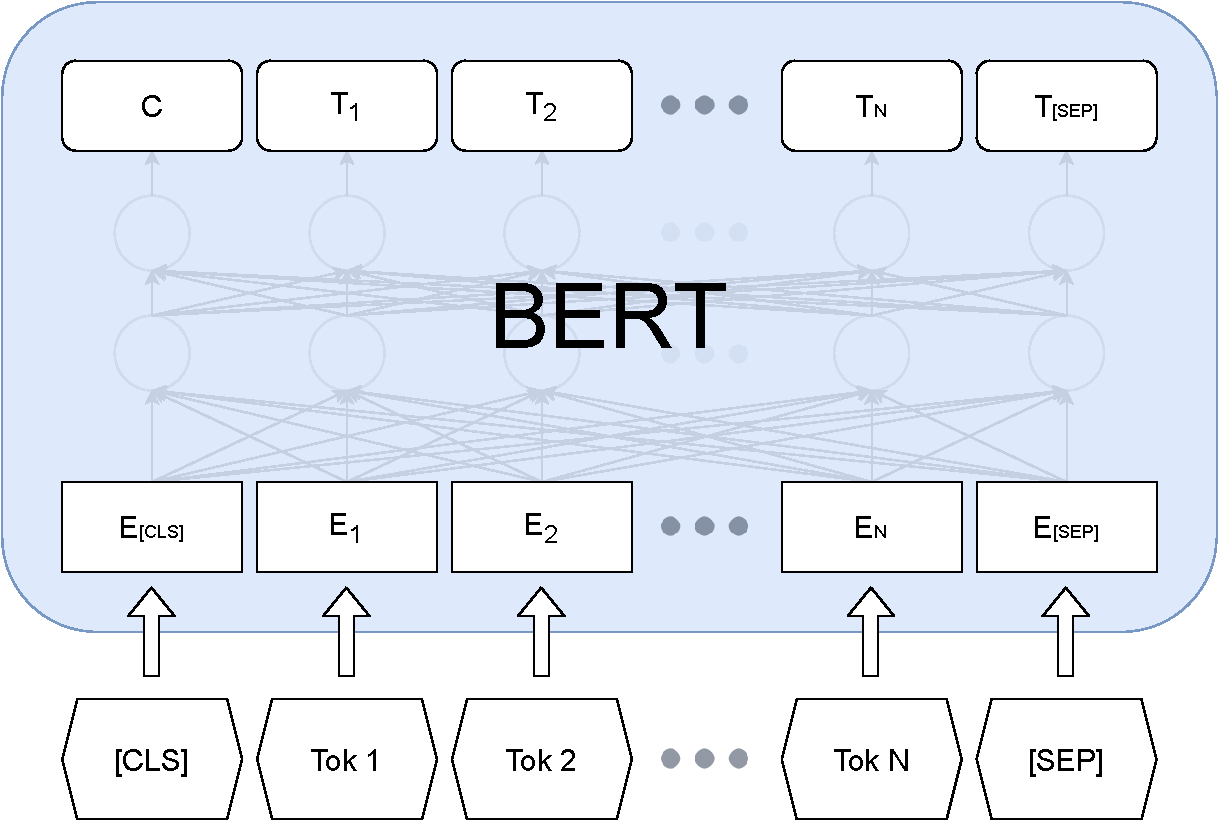
\includegraphics[width=\linewidth]{src/BERT.pdf}
	\caption{Schematic illustration of BERTs architecture. \newline Source: Adapted from \cite{Devlin2018}}
\end{figure}
BERT is a modern approach to create a model that can take into account the context of a word in both directions. Thus, the model would be better able to interpret words through their context. Based on this architecture, a model is then pretrained on a corpus using masklm and nextsentence tasks. This base model can then be used for new tasks with relatively little effort.

The Masklm task consists of masking random words in a sentence and having the model guess what the masked word actually was. This task is commonly referred to as masked ML task or MLM for short. For training the original BERT model, about 15\% of all input tokens are masked and by predicting the missing words, BERT is supposed to learn an understanding of natural language.

The Next Sentence Prediction task consists of inferring relationships between two sentences. Because this task is not covered by MLM. The Next Sentence Prediction, or NSP for short, is intended to teach the model of a given sentence following a previously given one by means of a binary classification task. Especially QA and NLI are supposed to benefit from this training. 

These two tasks were then used to train BERT on the BooksCorpus and on English Wikipedia texts. At this point, a pre-trained model is obtained, which can then be used in various ways depending on the particular task. Further training on a a new task is referred to as finetuning. 

Since finetuning tasks are quite specific, the details depend on the selected task. However, in general, the procedure can be classified into one of two groups. First, there are classification tasks based on complete sentences. These generally use the representation of the CLS token with a classifier layer. The other group of tasks operates at the token level and therefore uses the representation of the tokens using one or more additional layers. Once the architecture is set, the fine-tuning can take place. This is done end to end, so the whole transformer, i.e. BERT and the task specific part are tuned together. If BERT is not supposed to be changed, there is generally the possibility to freeze specific layers and thus prevent the change of weights in these. This leads to the fact that for example only the task specific part of the transformer is trained. 

%\begin{itemize}
%	\item BERT as revolution
%	\item pretrained-models
%	\item usefull even without finetuning
%	\item $\Rightarrow$ unexpected precision
%	\item nowadays used for many different NLP tasks
%	\item Architecture of BERT
%	\begin{itemize}
%		\item explain corpora
%		\item explain vocabulary
%		\item explain tokenizer
%	\end{itemize}
%	\item extensions of BERT like roBERTa
%\end{itemize}

\section{BioBERT}
BioBERT is one of the extensions of BERT which has emerged because BERT by itself did not yield the desired results in the biomedical landscape. This observation has often been related to the differences in word distributions between a general domain such as Wikipedia, on which BERT was trained and the highly specialized words that are used often or with this meaning only in the corresponding domain. This difference in the underlying corpora not only produces differences in the architecture of the model itself but implies a possible need for adjustments to the used vocabulary and the tokenizer. \cite{Lee2019} 
\newline
Based on this prior knowledge, it was hypothesized that a model that takes these particularities into account should perform significantly better than general models in tasks of this specific domain. Based on this hypothesis, BioBERT was created. A model that should be better adapted to the biomedical domain than BERT.
\newline
Nevertheless, BioBERT itself is only a further trained version of BERT. This means the original BERT model was used as the basis and further trained on either PubMed abstracts, PubMed central full-text articles, or on both. Therefore the authors chose to keep the original BERT vocabulary to be able to use the pretrained version of BERT as the basis. This had the advantage that the original model only needed to be further trained on the new corpus and the needed training time could be reduced. For the tokenizer WordPiece was used to handle the problem with unknown words. It was also considered to create a new vocabulary, but this idea was discarded in order to preserve the previously mentioned advantage of being able to utilize the pre-trained BERT model to save resources. 
As a result, it was observed that BioBERT performed better than BERT in version 1.0 that was based on PubMed abstracts and the full text articles of PubMed Central biomedical landscape with very few exceptions. Although the actual measured improvements sometimes vary quite significantly, it can be safely concluded that even continued training of BERT on a biomedical corpus can lead to significant improvements on tasks from this domain. 


\section{S2ORC-BERT}
S2ORC, known as the Semantic Scholar Open Research Corpus, is a corpus that contains a large number of papers as well as metadata and the references associated with the papers. According to the authors, the full text portion of the corpus alone is the largest structured academic text corpus available in April 2020. This corpus is based on semantic scholar papers and thus comes from several different origins. Although the main part of the paper is the acquisition and processing of papers and the resulting construction of the S2ORC corpus, the authors also use that corpus to continue training BERT. This is relatively reminiscent to the basic idea and the approach, which is also behind BioBERT, but in this case it is closer to the approach used for SciBERT. 

We will take a closer look at SciBERT at a later point in time. S2ORC-BERT, as the model trained here is called, unlike BioBERT, is trained from scratch and is therefore not based on the pretrained BERT model. Some important features are that the loss is calculated by cross entropy and the optimizer is Adam. The learning rate as well as the number of epochs per task are derived from two predefined sets. Here the combination is chosen that gives the best result for the respective task according to the development set. Since the S2ORC-BERT is rather used for validation of the corpus and clearly less focused on a new architecture for BERT, many parameters are identical to those of other papers, in particular the values reported for SciBERT were used. It should be mentioned that the difference between this model and BERT and SciBERT is almost exclusively due to the underlying corpus and the associated vocabulary.  




\section{AOG-BERT}
	Another approach that does not only aim at matching the corpus on which BERT is trained better to the later domain, but at the same time tries to teach the model a more extensive understanding of the texts is AOG-BERT. With this further goal, however, the training strategy underlying BERT needs to be adapted as well, because as we saw earlier, BERT's pre-training is based only on a Masklm task and a Nextsentence classification. Although these two tasks together ensure that we get a decent initial model, the question remains whether specific tasks can be solved better by a more specific training in the pre-training process or by embedding additional information.
	Based on this, one could argue that a model with domain entity knowledge could perform better than a model that does not use this information. For example, \citeauthor{Liu2021} argue that specific institutes may be more focused on specific scientific domains and that this knowledge could help the model to assign a paper to a research domain. Although it should be reasonable to assume that the actual text should be sufficient to assign a paper to a research area, this knowledge might prove beneficial for the model.
	

	Compared to existing approaches, OAG-BERT attempts to use not only homogeneous knowledge but also non-homogeneous knowledge from the Open Academic Graph. The information types used include authors, fields of study, venues and affiliation.
	
	To integrate this information into the model, three crucial changes are made compared to BERT.  
	
	The first adaptation is the heterogeneous entity type embedding. Here, the token type embeddings are replaced with entity type embeddings, providing unique labels for the different entity types, so that it is possible to identify which input belongs to which category.
	The next modification is the entity-aware 2D-positional encoding. Just like BERT, OAG-BERT needs positional embeddings to be aware of the sequence order. However, BERT does not have the ability to distinguish between two directly adjacent entities and would interpret them as one entity. To solve this problem, the positional embeddings in OAG-BERT are two dimensional and encode in the first dimension the so-called inter-entity sequence order and in the second dimension the intra-entity sequence order. (Final result is the sum of the two dimensions? )
	
	The last change is the span-aware entity masking. Although the masking strategy is not changed for either the abstract or the actual text, special masking is proposed for the new entity types. This is supposed to help OAG-BERT to learn complex entities especially if they consist of many tokens. This means that an entity consisting of four or less tokens is completely masked, but as soon as it is longer only a part of the entity is masked. Here the length of the mask is drawn from a geometric distribution.   
\color{ForestGreen}
\begin{itemize}
	\item als kontrahend zu SciBERT \cite{Liu2021}
\end{itemize}

\section{Datasets}
\begin{itemize}
	\item zum Beispiel NCBI-Disease (versuch einen goldstandard für corpora zu erstellen)
	\item sehr günstig um darauf entsprechende modelle zu trainieren \cite{Dogan2014}
	\item SciERC /sciie im repo \cite{luan2018multitask}
\end{itemize}
\color{black}
Due to the availability of the Datasets used by the original authors, we will use their prepared datasets, which are already prepared in a way that it is easier to use them for training and still only vary slightly from the original datasets. The datasets which we will use are directly retrieved from the SciBERT GitHub page and made available through the DataDeps package which provides an easy way to retrieve data that may or may not be locally available. If it is not already stored locally, it will be cached in the local Julia path and inside Julia, DataDeps provides the corresponding paths to the data and retrieves it from the defined source if needed. Furthermore, a hash can be defined as well to ensure that the provided data is identical to the expected one.\cite{White2019}\\
In the following paragraph, we will take a closer look at the original data and the individual changes that have been made to use those Datasets for the training process.
\subsection{Chemprot}
Chemprot is in a JSON lines file format provided. More precisely every line consists of a text and the corresponding label. A field for metadata exists as well but is most of the time not used. In its original format, the Chemprot corpus consists of a develop, test, and train set of which the develop, test, and train folder correspond to the identically named files inside the chemprot folder provided on the GitHub site of SciBERT. The difference arises from a database-like structure in which the Chemprot corpus is originally provided, in contrast to those subdivided information sets where for example the text itself is in another file than the positions and annotations. Those divided pieces of information were combined and are provided in a single file in the already mentioned format. \cite{Beltagy2019,Wang2016}